\chapter{Parameters identification}
\label{chap:paramidentification}
\section{Steady state analysis}
\label{sec:steadystate}
Using the data of the file, we analysed the step response of the system by going
to check the relationships between the stiffness of the springs. 
And estimating a new coefficient for the voltage-to-force.
The estimate of a new voltage-to-force coefficient is carried out using the 
equation:

and therefore from '22' it is possible to derive:

Using the steady state value of the three output and the equation '22' it is 
possible to evaluate the ratio of the stiffness of the springs with respect to 
the nominal value of the third spring indicated with 'k3', so it is possible to
rewrite:
\begin{equation}
	\label{eq:gvestimate}
	\begin{bmatrix}
		gain_v + (gain_v*k3)/k1 + (gain_v*k3)/k2
    		gain_v + (gain_v*k3)/k2
    		gain_v
    \end{bmatrix}
\end{equation}


\begin{table}[ht]
\centering
	\begin{tabular}{lrrr}
	\toprule
						& nominal & computed & error [\%] \\
 	\midrule
 	ratio $k_{3}/k_{1}$	& 0.50000 & 0.48935 &	2.17651 \\
	ratio $k_{3}/k_{2}$	& 0.50000 & 0.52086 & 	4.00560 \\
	gain ratio			& 5.25000 & 6.04866 &  15.21248	\\
	\bottomrule
	\end{tabular}
\caption{Stiffnesses ratios and voltage-to-force coefficients}
\label{tab:erro}
\end{table}
%
%%%%%%%%%%%%%%%%%%%%%%%%%%%%%%%%%%%%%%%%%%%%%%%%%%%%%%%%%%%
%
\section{System identification}
\label{sec:sysidentification}
It is necessary to estimate the parameters of a 3 \textsc{dof} system at simple 
identification, so that the impulse response is used to suppose that a model is 
based on a set of parameters, identifying the inputs as the initial force and 
conditions and the output of the system.
thus comparing the system response measured with that predicted by the model.


Defined a model for the system: depends on a set of parameters $\theta$. 
Identify the input (strength and i.c.) and output $(x(t))$ of the system. 
By giving the same input to the model and comparing the measured response $x(t)$ 
to that expected by the model $(x(t,\theta))$.
%
\begin{figure}[h]
\centering
\begin{tikzpicture}
% help guide lines
%\draw[help lines] (0,0) grid [step = 5 mm](10,10);
%\foreach \x in {0,1,...,10}
%   \draw [help lines] (\x,0) node [below,%
%          font=\footnotesize] {$\x$} -- (\x,0);
%\foreach \y in {0,1,...,10}
%   \draw [help lines] (0,\y) node [left,%
%          font=\footnotesize] {$\y$} -- (0,\y);
%
% define model box
\newcommand{\modelbox}[2]{
	% input arrow  
	\coordinate (startarrow) at ({#1},{#2});
	\coordinate	(endarrow) at ($(startarrow)+(2.5,0)$);
	\draw [-stealth]($(startarrow) + (0,1 * 1)$) -- ($(endarrow)+(0,1* 1)$) node[above, midway] {$f(t)$};
	\draw [-stealth]($(startarrow) + (0,1 * 0)$) -- ($(endarrow)+(0,1* 0)$) node[above, midway, xshift=-0.65mm] {$\vec{x}_{0} \,, \dot{\vec{x}}_{0}$};
	% box
	% left low corner
	\coordinate (llcorner) at (2.5,-0.5);
	% right up corner
	\coordinate (rupcorner) at(6.5,1.5);
	\draw (llcorner) rectangle (rupcorner) node [midway]{dynamic system};
	% output arrow
	\coordinate (outputstartarrow) at (6.5,0.5);
	\coordinate	(outputendarrow) at (8.5,0.5);
	\draw [-stealth](outputstartarrow) -- (outputendarrow) node[above, midway] {$\vec{x}(t)$};
};
% 1 - plot the system model
\begin{scope}[yshift = 60mm]
   \modelbox{0}{0};  
\end{scope}
% 2 - plot second model and connection
\begin{scope}[yshift = 25mm]
   \modelbox{0}{0};
   \fill (1.75,1) circle (1.4pt);
   \fill (1,0) circle (1.4pt);
\end{scope}
% connect system model
   \draw (1.75,1) -- (1.75,3.5);
   \draw (1,2.5) -- (1,0);
% box model
\begin{scope}[xshift = 0mm]
   % input arrow  
	\coordinate (startarrow) at (1.75,1);
	\coordinate	(endarrow) at (2.5,1);
	\draw [-stealth](startarrow) -- (endarrow) node[below, midway] {$f(t)$};
	\draw [-stealth](1,0) -- (2.5,0) node[below, midway] {$\vec{x}_{0} \,, \dot{\vec{x}}_{0}$};
	% box
	% left low corner
	\coordinate (llcorner) at (2.5,-0.5);
	% right up corner
	\coordinate (rupcorner) at(6.5,1.5);
	\draw (llcorner) rectangle (rupcorner) node [midway]{model $\theta$};
	% output arrow
	\coordinate (outputstartarrow) at (6.5,0.5);
	\coordinate	(outputendarrow) at (8.5,0.5);
	\draw [-stealth](outputstartarrow) -- (outputendarrow) node[above, midway] {$\vec{x}(t)$};
\end{scope}
\end{tikzpicture}
\label{fig:systemmodel}
\caption{System identification: real system and model}
\end{figure}
%
We define the residue as the difference between the two signals as in the 
equation (\ref{eq:residual}).
\begin{equation}
\label{eq:residual}
	\varepsilon(t,\theta) = x(t) - x(t,\theta)
\end{equation} 
The best choice for the set of parameter $\theta$ is the one that minimizes the 
residue integer (\ref{eq:residualinteger}) of the residue. 
\begin{equation}
\label{eq:residualinteger}
	\theta_{optim} = \text{argmin} \biggl( \int \varepsilon(t,\theta)^2 \, dt \biggr)
\end{equation} 
In this case, as the discrete signals with $N$ samples, the optimal value $N$ 
calculated as (\ref{eq:residualdiscrete}), this correspond to solving a least 
square problem.
\begin{equation}
\label{eq:residualdiscrete} 
\theta_{optim} = \text{argmin} \Biggl( \sum_{n=1}^{N} \varepsilon(t,\theta)^2 \Biggr)
\end{equation}

A linear model is adopted as described above, refer \ref{subsec:assumption}, 
assuming the stiffness matrix $[K]$ given.
Then quantifying the $[M]$ and $[C]$ parameters are used to minimize the problem.
Using the \emph{fmincon} algorithm, the problem is resolved. In addition, the 
selected algorithm is required to specify the lower and upper search limits; 
as well as the first guess conditons from which the result is strictly dependent.

\subsection{Free damping case}
\label{subsec:freedamping}
The estimation is performed using the model in equations, the parameters to 
estimate are 7. The results are shown in table \ref{tab:freedamping}.
\begin{table}[ht]
\centering
\begin{tabular}{SSSSSSS}
	\toprule
\multicolumn{1}{c}%
		{$m_1$} & {$m_2$} & {$m_3$} & {$c_1$} &	 {$c_2$} & {$c_3$} & {$g_v$} \\
\multicolumn{3}{c}{[\si{\kilo\gram}]}	&%
\multicolumn{3}{c}{[\si{\newton\second\per\meter}]}	&%
\multicolumn{1}{c}{[\si{\volt}]}\\
	\midrule
          1.5712  & 1.5020  & 1.2018  &  2.7956 &  1.9978 & 2.1950  &  1.2096	\\
    \bottomrule
\end{tabular}
\caption{Optimizations results in free damping case}
\label{tab:freedamping}
\end{table}
%
\begin{figure}[h]
\centering
	\subfloat[][\emph{residual.}]
	{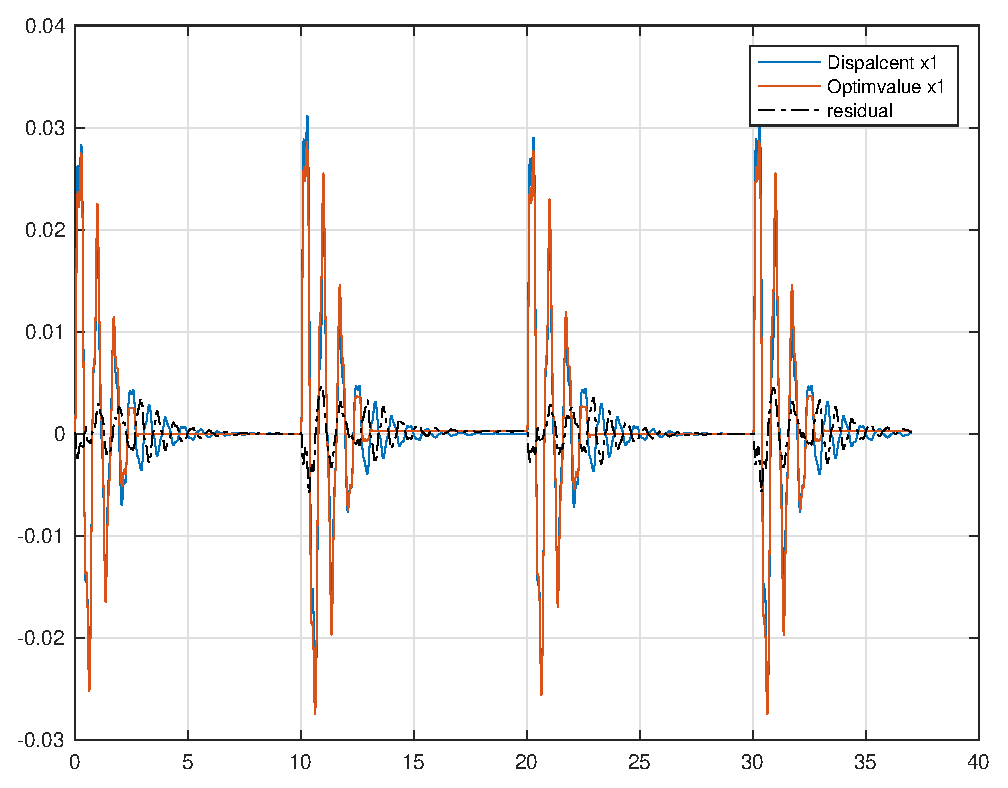
\includegraphics[width=0.55\textwidth]{residualfull1}}	\\
	\subfloat[][\emph{residual.}]
	{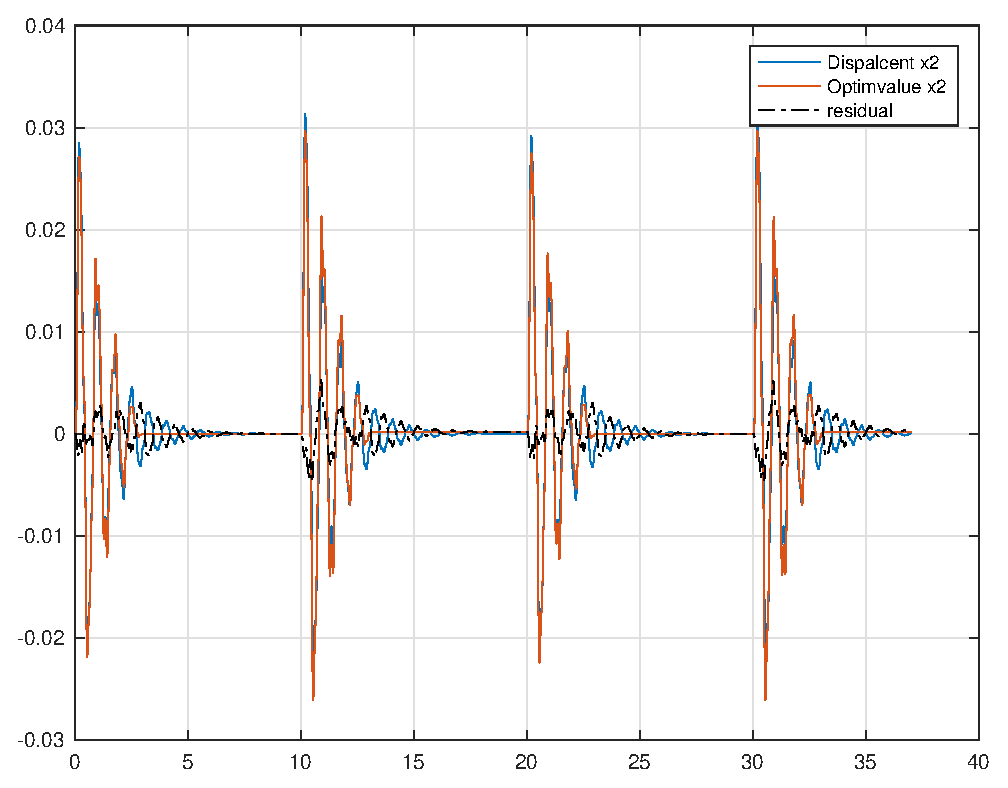
\includegraphics[width=0.55\textwidth]{residualfull2}}	\\
	\subfloat[][\emph{residual.}]
	{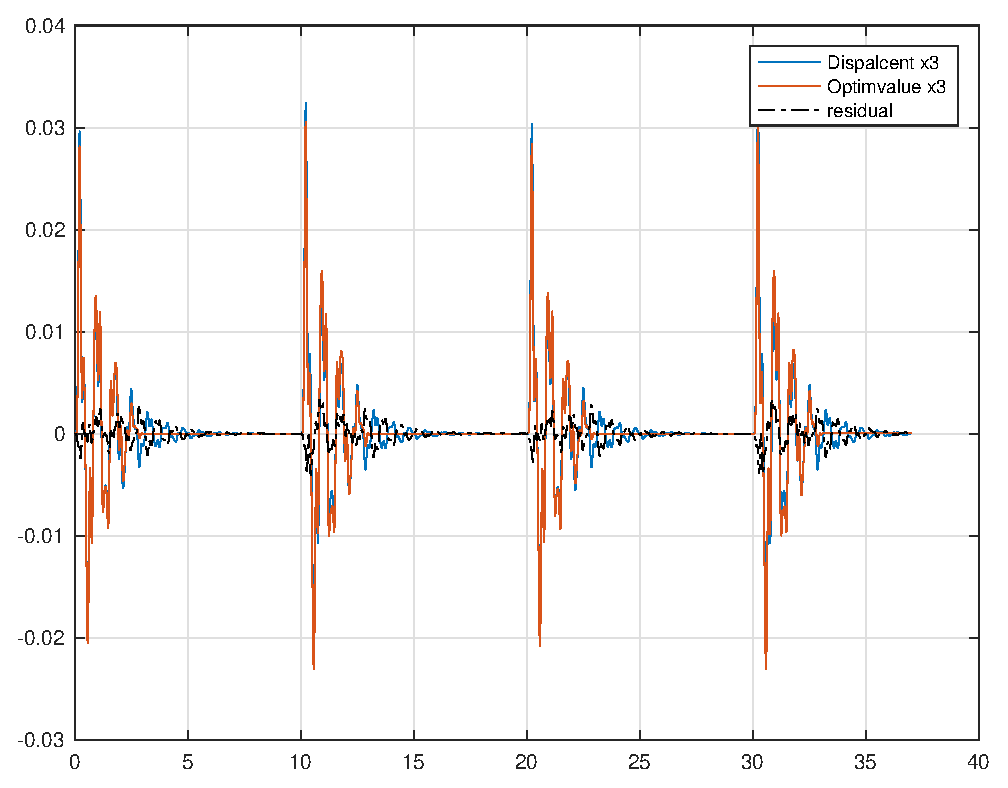
\includegraphics[width=0.55\textwidth]{residualfull3}}	\\
	\caption{Comparison between the response of the model and the response of the 
	system free damping case}
	\label{fig:freedampingcase}
\end{figure}
%
\clearpage
%
\subsection{Proportional damping case}
\label{subsec:proportionaldamping}

In this case, the procedure used to solve the problem raised in the case of 
free damping to obtain the parameters is used; changing some conditions.
We define damping through the equation (\ref{eq:proportionaldamping}) where it 
is possible to observe that this depends on the linear combination of the mass 
matrix multiply by constant and the stiffness matrix multiply by the another 
constant.
Then the search limits and first guess will be changed to search the mass 
values and the unknown costants.
The interesting property of this representation is the ability to perform modal 
decomposition on the system.
\begin{equation}
\label{eq:proportionaldamping}
	[C] = \alpha \cdot [M] + \beta \cdot [K]
\end{equation}
The optimization results are available in the table \ref{tab:proportionaldamping}.
%
\begin{table}[ht]
\centering
\begin{tabular}{SSSSSS}
	\toprule
\multicolumn{1}{c}%
			{$m_1$} & {$m_2$} & {$m_3$} & {$g_v$} &	 {$\alpha$} & {$\beta$} \\
\multicolumn{3}{c}{[\si{\kilo\gram}]}	& %
\multicolumn{1}{c}{[\si{\volt}]} & %
\multicolumn{2}{c}{[\si{\newton\second\per\meter}]} \\
	\midrule
       			1.5761   &  1.4970  & 1.1996  &  1.2094 &  1.6209   &  0.0001	\\
    \bottomrule
\end{tabular}
\caption{Optimizations results in proportional damping case}
\label{tab:proportionaldamping}
\end{table}
%
%
%
\begin{figure}[ht]
\centering
	\subfloat[][\emph{residual.}]
	{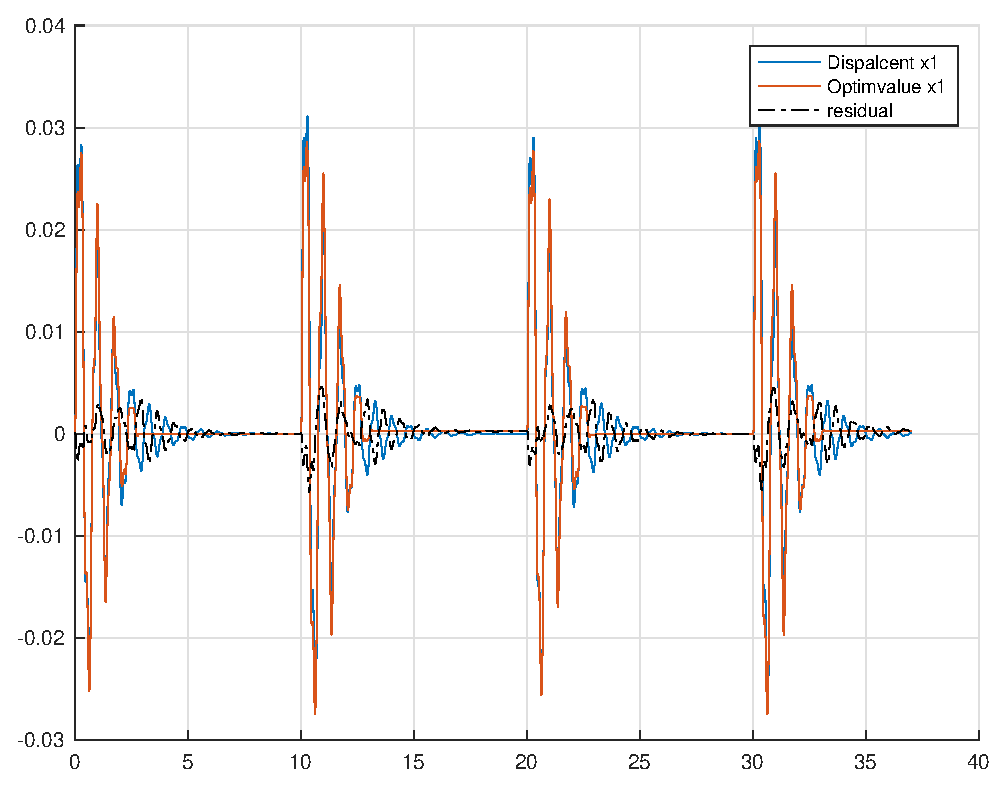
\includegraphics[width=0.55\textwidth]{residualpropdamp1}}	\\
	\subfloat[][\emph{residual.}]
	{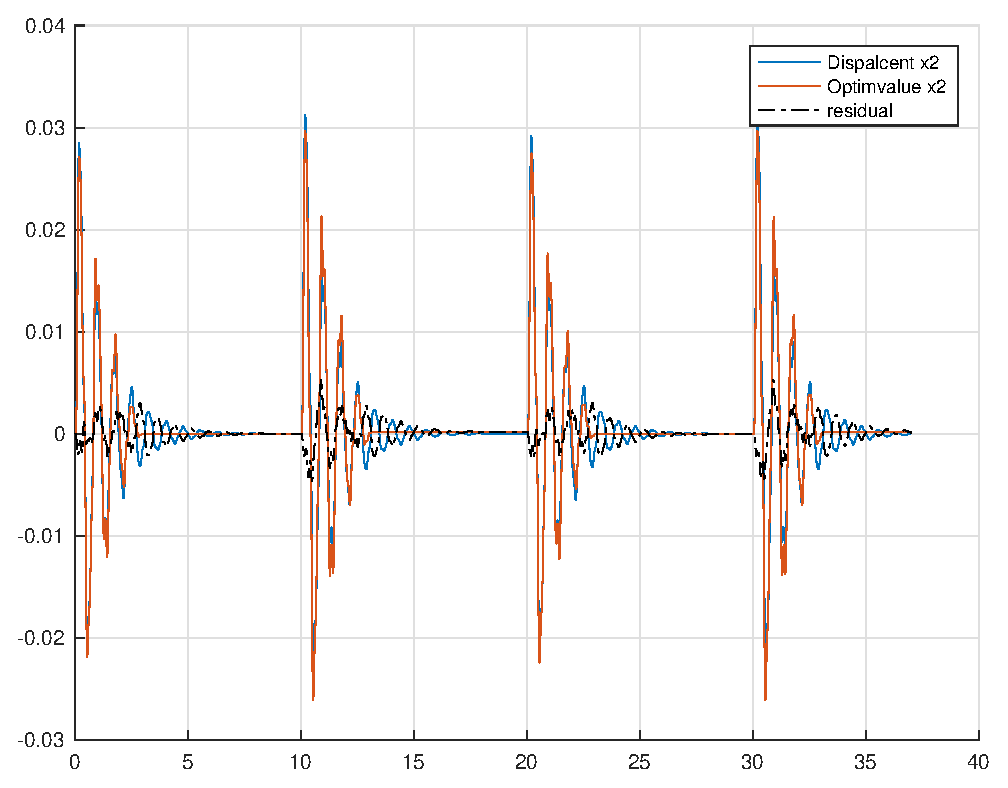
\includegraphics[width=0.55\textwidth]{residualpropdamp2}}	\\
	\subfloat[][\emph{residual.}]
	{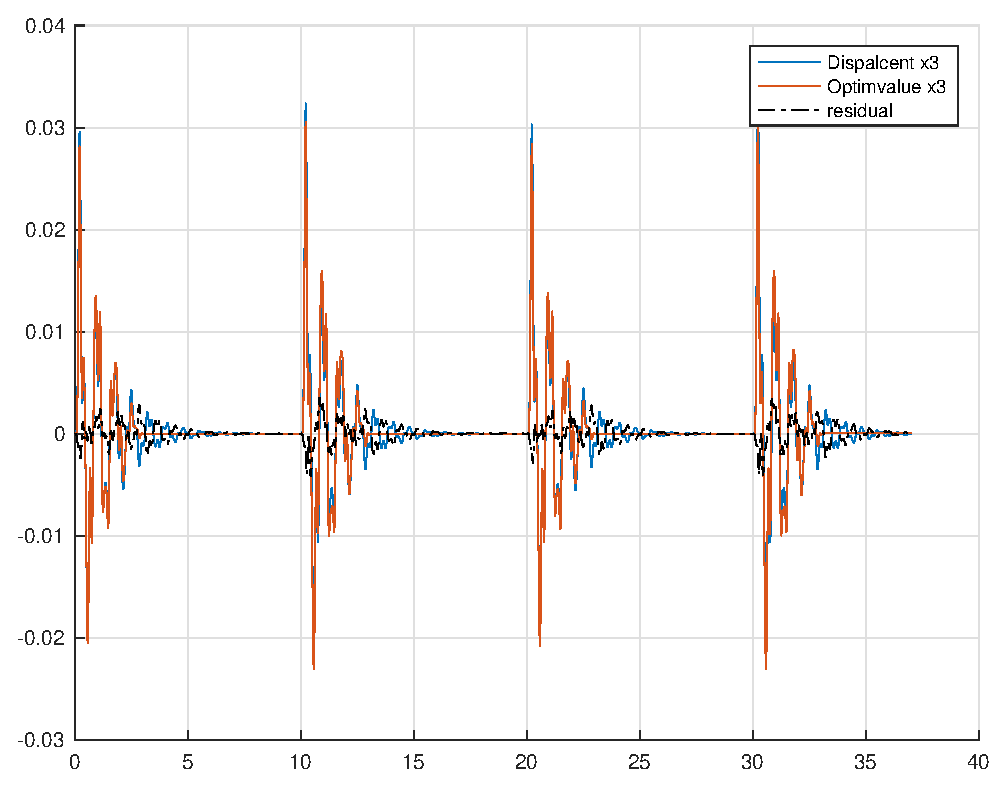
\includegraphics[width=0.55\textwidth]{residualpropdamp3}}	\\
	\caption{Comparison between the response of the model and the response of the system proportional damping case}
	\label{fig:proportionaldamping}
\end{figure}
%
%
%
%
%%
%TODO describe the matrix C 
%The matrix [C] is:
\begin{equation}
\label{}
	[C] =
	\begin{bmatrix*}[r]
		 2.64026		&	-0.08550		 & 	 0.00000 	\\
		-0.08550 	&	 2.59748		 &	-0.08550		\\
		 0.00000 	&	-0.08550		 &	 2.07270		\\
	\end{bmatrix*}
\end{equation}
%
\subsection{Comparison}
\label{subsec:comparison}
After fitting data with a model, you should evaluate the goodness of fit. 
The goodness of fit is calculated using the normalized root mean square error 
as the cost function.
In table \ref{tab:goodoffit} are aviable the percentages the measured output.
This method to assess goodness of fit for both linear and nonlinear parametric 
fits.
As is common in statistical literature, the term goodness of fit is used here 
in sense:  ``good fit" might be a model where the data could reasonably have 
come from, given the assumptions of least-squares fitting.
\begin{table}[ht]
\centering
\begin{tabular}{lccc}
	\toprule
		 & $x_1$ [\%] & $x_2$ [\%] & $x_3$ [\%]\\
	\midrule
	% free damping result
	free damping case & 81.36 & 81.17 & 81.71 \\
	% proportianl damping result
	proportinal damping case & 81.36 & 81.17 & 81.56 \\
	\bottomrule
\end{tabular}
\caption{Result \emph{goodness of fit} measured output}
\label{tab:goodoffit}
\end{table}
%
%
%
%
%
%\section{Occorrente}
%\label{sec:occorrente}
%
%Roba da scaricare e installare (Tabella \ref{tab:filesize}).
%
%\begin{table}[h]
%\centering
%\caption{Tabella vergognosamente inutile}
%\vspace{0.3cm}
%\label{tab:filesize}
%\begin{tabular}{lll}
% \hline
%File & Piattaforma & Dimensioni \\\hline
%\emph{TexMaker} & Windows & 46.3 MB \\
%\emph{TexMaker} & Mac & 40.7 MB \\
%\emph{MiKTeX} & Windows & 154.1 MB \\
%\emph{MacTex} & Mac & 2.3 GB \\
%Template Susanna & Multiglobale-powa & 4 MB (circa) \\\hline
%\end{tabular}
%\end{table}
%
%\pagebreak
%
%%%%%%%%%%%%%%%%%%%%%%%%%%%%%%%%%%%%%%%%%%%%%%%%%%%%%%%%%%%%
%
%\subsection{L'IDE}
%\label{sub:ide}
%
%Allora... per prima cosa vi serve un IDE, ovvero un programma che vi funga da editor e compilatore (in realtà il compilatore si scarica a parte ma vabbè). Ce ne sono molti in giro ma io vi consiglio \emph{TexMaker}\footnote{http://www.xm1math.net/texmaker/} per due motivi:
%
%\begin{enumerate}
%\item È molto intuitivo è ben fatto
%\item Esiste sia per Mac che per Windows
%\end{enumerate}
%
%Non dovreste avere problemi con il download e l'installazione (vi state per laureare porca paletta, non devo spiegarvi pure questo).
%
%%%%%%%%%%%%%%%%%%%%%%%%%%%%%%%%%%%%%%%%%%%%%%%%%%%%%%%%%%%%
%
%\subsection{Il compilatore}
%\label{sub:compilatore}
%
%Per quanto riguarda il compilatore il discorso è un po' più complicato. Armatevi di pazienza e scaricate \emph{MiKTeX}\footnote{http://miktex.org/download} se avete Windows oppure \emph{MacTex}\footnote{http://mirror.ctan.org/systems/mac/mactex/MacTeX.pkg} se avete un Mac (mi dispiace ma non conosco un compilatore LaTeX per Linux... se lo trovato fatemelo sapere che aggiorno la guida). Entrambi questi programmi inglobano un ambiente di sviluppo \LaTeX costituito da diversi compilatori che il nostro IDE riconoscerà automaticamente.
%
%\textbf{P.S.} Prima che cominciate a strapparvi i capelli, sì, \emph{MacTex} occupa più di 2 GB... questo perchè comprende tutti i pacchetti necessari per \LaTeX, mentre \emph{MiKTeX} (che occupa solo 150 mb) li scarica volta per volta.
%
%%%%%%%%%%%%%%%%%%%%%%%%%%%%%%%%%%%%%%%%%%%%%%%%%%%%%%%%%%%%
%
%\subsection{Il template}
%\label{sub:template}
%
%Trovate il sorgente di questo template ad un link dropbox non meglio specificato\footnote{https://www.dropbox.com/sh/1f06sd7eprongvl/dKsfID1Kwc}
%
%%%%%%%%%%%%%%%%%%%%%%%%%%%%%%%%%%%%%%%%%%%%%%%%%%%%%%%%%%%%
%
%\section{Configurazione dell'IDE}
%\label{sec:configurazioneIDE}
%
%Oooh, ora che avete installato IDE e compilatore, lanciate l'IDE. Principalmente dovete fare tre cose una volta avviato:
%
%\begin{enumerate}
%\item Aprite il file Susanna.tex del template
%\item Andate su Opzioni -> Definire il documento corrente come Master (questo serve per dire all'IDE che gli altri documenti sono inclusi in un documento master e che quindi, al momento della compilazione, non devono essere trattati come documenti separati)
%\item Andate nelle preferenze dell'IDE nella sezione Compilazione Rapida e personalizzate la compilazione tramite l'assistente-wizard. Essenzialmente dovete configurarla in modo da effettuare 3 compilazioni: PdfLatex, BibTex e di nuovo PdfLatex. Oltre a queste tre compilazioni aggiungete una quarta opzione ovvero la visualizzazione pdf.
%\end{enumerate}
%
%Vi spiego meglio il punto 3... praticamente ci sono più compilatori diversi, che svolgono operazioni diverse... ma a noi interessano solo due compilatori, ovvero PdfLatex (che compila il codice \LaTeX in un documento pdf) e BibTex (che compila la bibliografia). Le compilazioni sono 3 e in quel preciso ordine perchè altrimenti la bibliografia non viene compilata bene (non chiedetemi perchè). Per evitare di dover eseguire manualmente le diverse compilazioni, \emph{TexMaker} vi dà la possibilità di utilizzare la Compilazione Rapida che esegue automaticamente queste operazioni con un click. Configuratela come vi ho spiegato e non avrete problemi.
%
%%%%%%%%%%%%%%%%%%%%%%%%%%%%%%%%%%%%%%%%%%%%%%%%%%%%%%%%%%%%
%
%\section{Siamo pronti}
%\label{sec:pronti}
%
%Abbiamo configurato l'IDE ed il (i) compilatore(i). Ora premendo sulla freccina della Compilazione Rapida (oppure premendo F1) potrete compilare il vostro codice \LaTeX in pdf. Fate una prova compilando il template (il pdf purtroppo, così come tutti gli scarti della compilazione, verranno generati nella stessa cartella del sorgente...).
%
%E ora? Ora create i vostri capitoli copiando la struttura di \emph{start.tex} e di \emph{introduzione.tex} ed integrateli nel documento master :) se avete bisogno di ulteriori dettagli sulla sintassi \LaTeX vi consiglio di farvi un giro nella sezione Tex di \emph{Stack Exchange}\footnote{http://tex.stackexchange.com/}: è tipo Yahoo Answers ma focalizzato ovviamente su \LaTeX :)
